\documentclass{article}
\usepackage[T1]{fontenc}
\usepackage[utf8]{inputenc}
\usepackage[brazil]{babel}

\usepackage{graphicx}
\usepackage{listings}

\lstset{
    basicstyle=\ttfamily
}

\newcommand{\KNNL}{{\lstinline"KNNL"}}
\newcommand{\opencv}{{\lstinline"opencv"}}

\begin{document}

\title{
    INE5443 --- Reconhecimento de Padrões\\
    Aprendizado de uma paleta de cores por uma rede de Kohonen
}
\author{
    Tiago Royer --- 12100776
}

\maketitle

\section{Problema}

O objetivo era fazer com que uma rede de Kohonen aprendesse uma paleta de cores.

As redes de Kohonen são compostas por uma camada de entrada e uma camada interna;
elas não possuem saída.
Eu coloquei três nodos na camada de entrada;
estes nodos representam as intensidades dos componentes vermelho, verde e azul
na cor que está sendo fornecida na entrada.
A quantidade de nodos na camada interna pode ser definida pelo usuário.

Existe uma conexão entre cada nodo na entrada e cada nodo na camada interna.
Estas conexões foram utilizdas para criar uma visualização da rede.
Um exemplo de execução está disponível na imagem \ref{demo1}.

\begin{figure}[h]
    \centering
    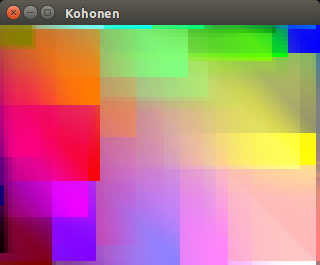
\includegraphics[scale=0.5]{demo1.png}
    \caption{
        Imagem gerada com o comando
        \texttt{./main --size 60 80 --input color\_list.txt --epochs 30 --seed 753}.
    }
    \label{demo1}
\end{figure}

\section{Detalhes da Implementação}

Para implementar as redes neurais, eu utilizei a biblioteca \KNNL.
É uma biblioteca para redes de Kohonen implementada em C++.
Ela é implementada inteiramente em headers
e é distribuída junto do código fonte do programa.

Esta biblioteca é altamante templatizada.
A própria escolha das funções de ativação dá-se via templates.
Portanto, cada combinação de algoritmo de treinamento,
tipo de rede, topologia, função de ativação etc.\ exige
que o programa seja recompilado com as novas especificações.
Por simplicidade,
fiz algumas escolhas arbitrárias,
que ficaram \emph{hardcoded} em minha aplicação.

Em particular, o algoritmo de aprendizado escolhido foi o
\emph{Winner Takes Most} (WTM),
numa rede neural retangular com métrica de Manhattan.

O \opencv foi utilizado para visualização.

\subsection{Interface com o usuário}

O programa possui várias opções de linha de comando;
um resumo delas pode ser obtido invocando \lstinline"./main --help".
Em particular, pode ser alterado
o tamanho da rede,
a quantidade de épocas de treinamento,
o valor inicial e a ``taxa de decaimento'' do raio de influência,
as cores a serem treinadas
e a semente inicial.
O arquivo \lstinline"run.sh" possui todos os exemplos de invocação
apresentados neste relatório.

Todas as opções possuem valores padrão,
portanto apenas invocar \lstinline"./main" funciona.

A opção \lstinline"--input" permite escolher quais cores
serão aprendidas pela rede neural.
O formato de arquivos foi projetado
para simplificar o parsing via \lstinline"std::istream";
é apenas uma lista de valores separados por espaços
(não por vírgulas)
correspondendo às componentes vermelho, verde e azul das cores escolhidas.
Dois exemplos são distribuidos com o programa
--- \lstinline"rgb.txt", com apenas as três cores primárias,
e \lstinline"color_list.txt", com 27 cores no total.

Uma combinação interessante é \lstinline"--seed" e \lstinline"--delta".
A primeira opção fornece uma semente ao invés de gerar uma;
a segunda opção escolhe a ``taxa de decaimento''
do raio de influência controlado pelo Winner Takes Most.
Como a semente não influencia o algoritmo de treinamento,
é possível ver, com pouca interferência externa,
o que uma maior ou menor taxas de decaimento fazem.

\end{document}
